\chapter{Circular motion}

\section{Pendulum on a peg}
\begin{wrapfigure}{o}{0.5\textwidth}
  \centering
  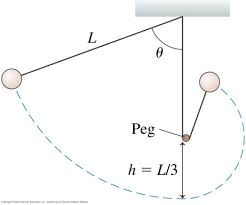
\includegraphics[width=0.47\textwidth]{assets/balpeg.png}
  \caption{Pendulum with peg attached}
  \label{fig:balpeg}
\end{wrapfigure}
\begin{problem}
  A pendulum is formed from a small ball of mass \(m\) on a string of
  length \(L\), as in \cref{fig:balpeg}. A peg is placed at a height
  \(h = \lf{L}{3}\) above the lowest point of the pendulum. From what
  minimum angle \(\theta\) must the pendulum be released in order for
  the ball to go over the top of the peg without the string going slack?
\end{problem}

Treat points \(A\) and \(B\) as the point of release
and highest point the pendulum reaches after passing the peg.

Since no external forces act on the pendulum, energy is conserved
throughout the ball's motion, according to the \term{principle of
conservation of energy}. The loss in potential energy is equal to the
gain in kinetic energy.
\begin{equation*}
  E_A = E_B
\end{equation*}
Let the height from which the ball is released (w.~r.~t. its lowest
point) be \(H\); the potential energy at point \(A\) is \(mgH\).
Since the ball starts from rest, its kinetic energy at point \(A\) is \(0\).

At point \(B\), the ball would have incurred some gravitational
potential energy by rising through a height of \(2h=\f{2L}{3}\),
while also maintaining a non-zero velocity. This non-zero velocity
\(v_B\) is contributed only by the weight of the ball (and not the
tension in the string), so \(F_c = \f{mv_B^2}{r} = mg\) means that
\(v_B^2 = rg = \f{gL}{3}\).
\begin{align*}
  E_A &= E_B\\
  \cancel{m}gH &= 2\cancel{m}gh + \f{\cancel{m}v_B^2}{2} \\
  \cancel{g}H &= \f{2\cancel{g}L}{3} + \f{\cancel{g}L}{6}
\end{align*}
We get a neat relation, \cref{eq:handl}.
\begin{equation}
  \label{eq:handl}
  H = \f{5L}{6}
\end{equation}
The height the ball falls through is \(H = L - L\cos\theta =
L\ab(1-\cos\theta)\). Equating this with \cref{eq:handl}, we get
\begin{align*}
  H = \f{5L}{6} &= L\ab(1-\cos\theta) \\
  \cos\theta &= \f{1}{6} \\
  \theta &= \arccos\f{1}{6} \approx \hil{\qty{80.4}{\degree}}
\end{align*}
